\documentclass[aspectratio=169, xcolor=table]{beamer}

\usepackage{calc}
\usepackage{graphicx}
\usepackage{mathtools}
\usepackage{siunitx}

\graphicspath{{./images}}
\setbeamertemplate{navigation symbols}{}

\author{Chris Doble}
\date{}
\subtitle{Building a GPS receiver from scratch}
\title{Part 8: Solving}
\usetheme{Madrid}

% Show the topics frame at the start of each section
\AtBeginSection[]
{
  \begin{frame}
    \frametitle{Topics}
    \tableofcontents[currentsection, subsubsectionstyle=hide]
  \end{frame}
}

% Show the topics frame at the start of each subsection
\AtBeginSubsection[]
{
  \begin{frame}
    \frametitle{Topics}
    \tableofcontents[currentsection, currentsubsection, subsubsectionstyle=hide]
  \end{frame}
}

\begin{document}

\frame{\titlepage}

\section{The pseudorange equation}

\begin{frame}
  \frametitle{Coordinate system}

  \centering
  \only<1>{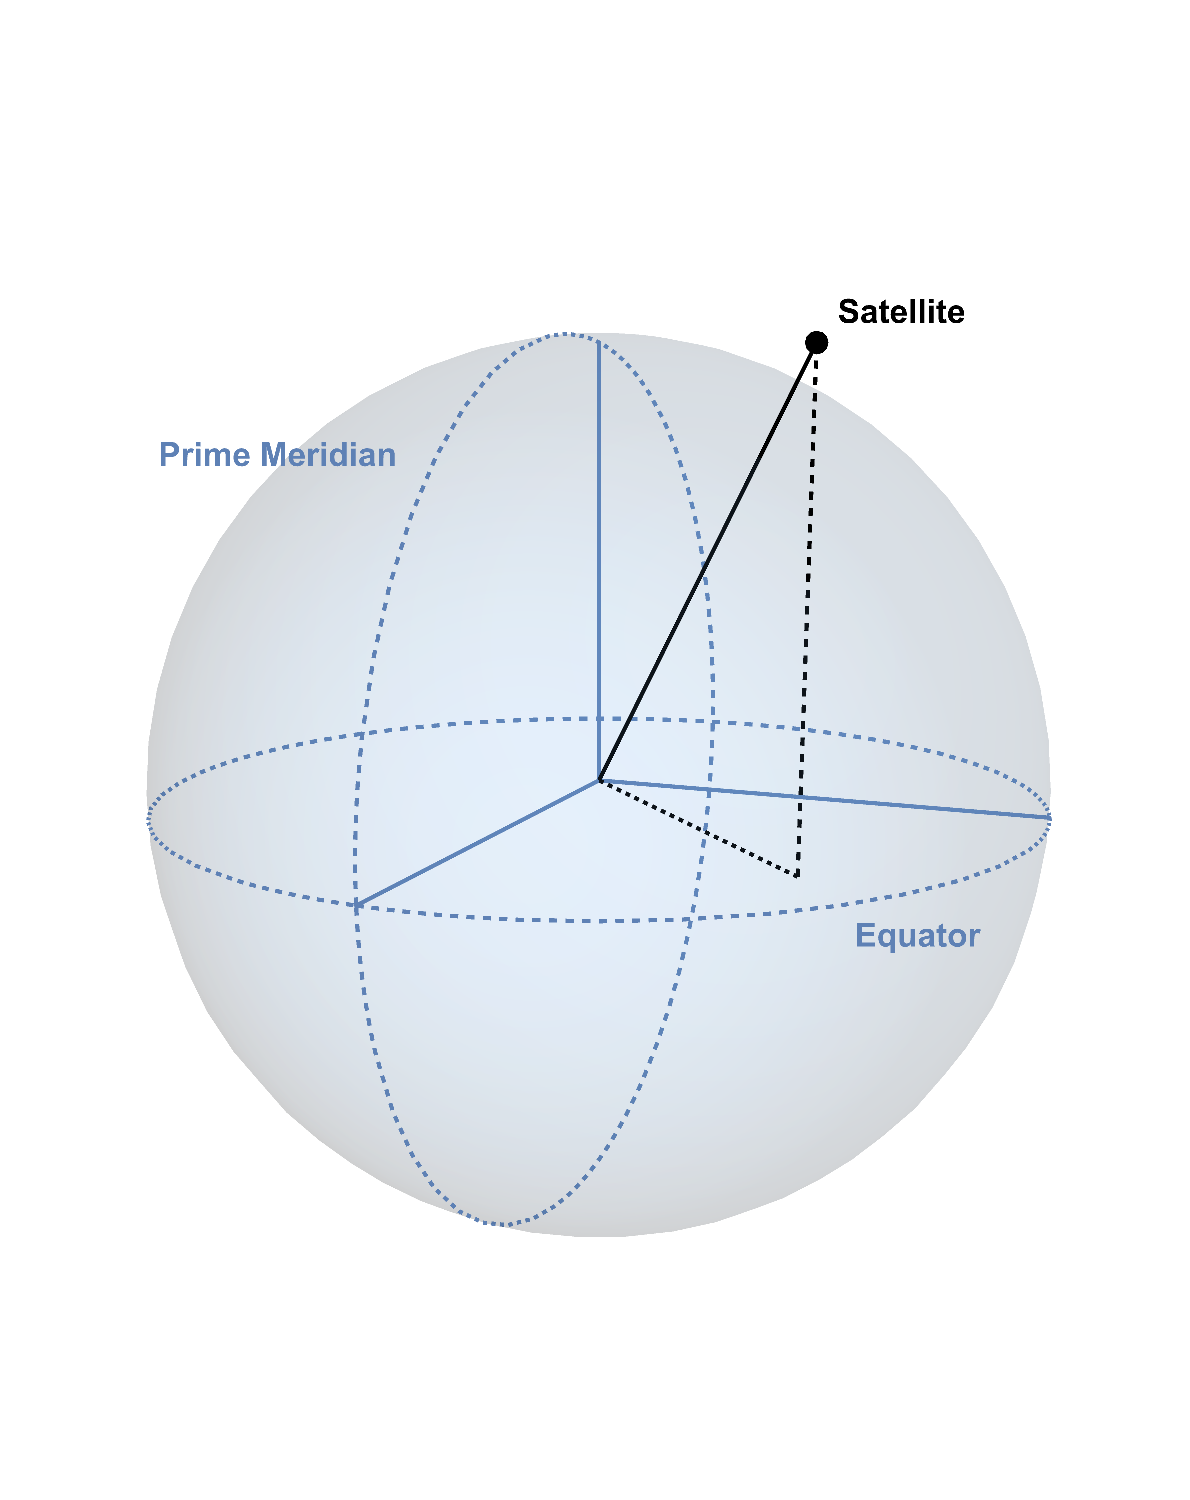
\includegraphics[clip, trim={2.4cm 4.4cm 1.6cm 3.5cm}, width=\textwidth * 35 / 100]{1 no coordinate system.pdf}}%
  \only<2>{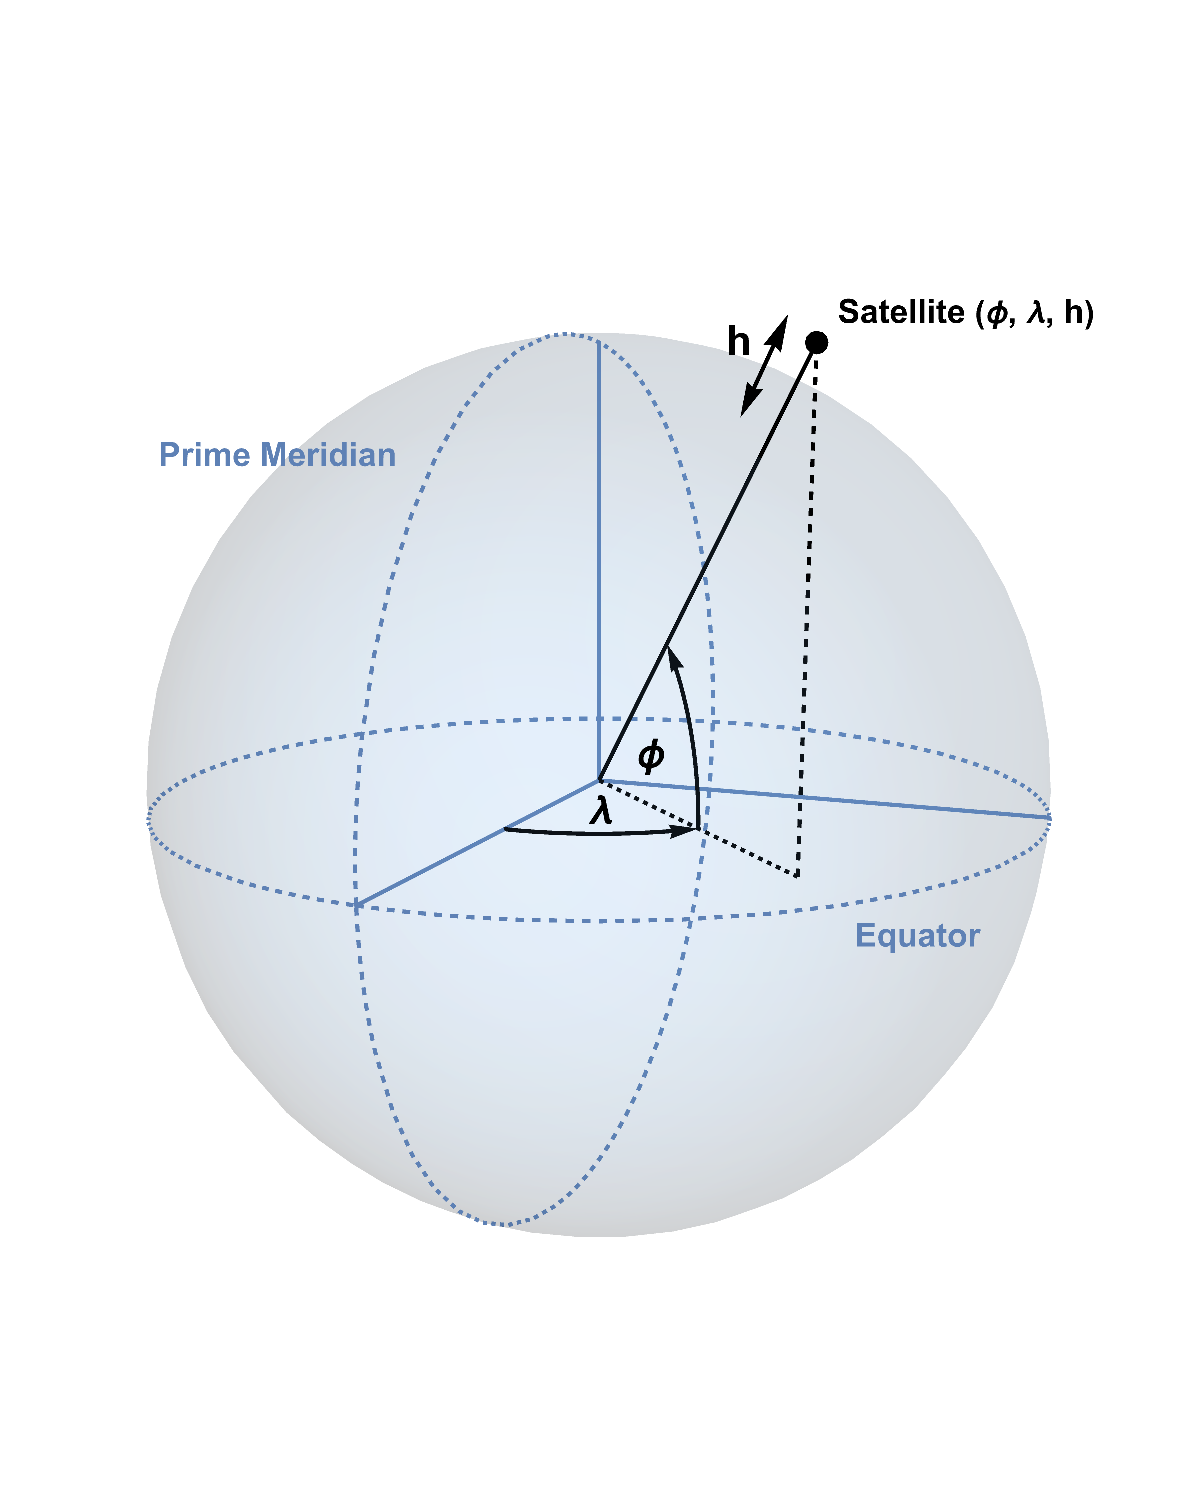
\includegraphics[clip, trim={2.4cm 4.4cm 1.6cm 3.5cm}, width=\textwidth * 35 / 100]{2 geodetic.pdf}}%
  \only<3-5>{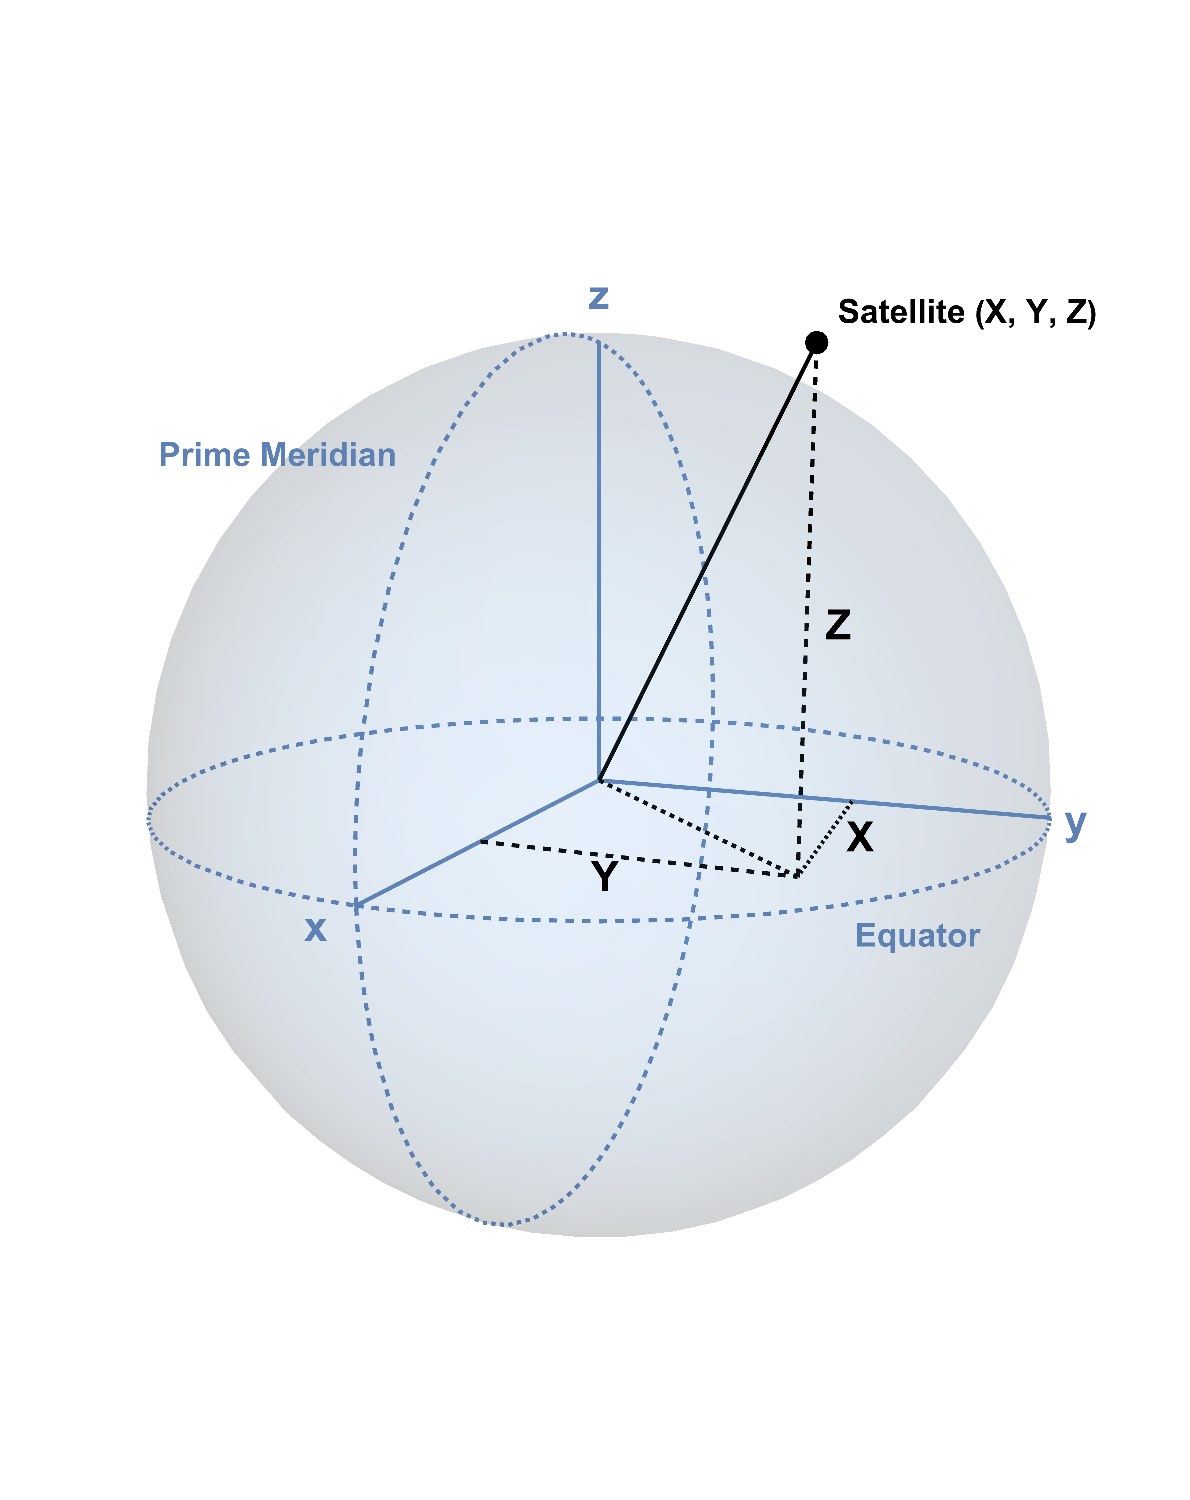
\includegraphics[clip, trim={2.4cm 4.4cm 1.6cm 3.5cm}, width=\textwidth * 35 / 100]{3 ecef.pdf}}%
  \only<6>{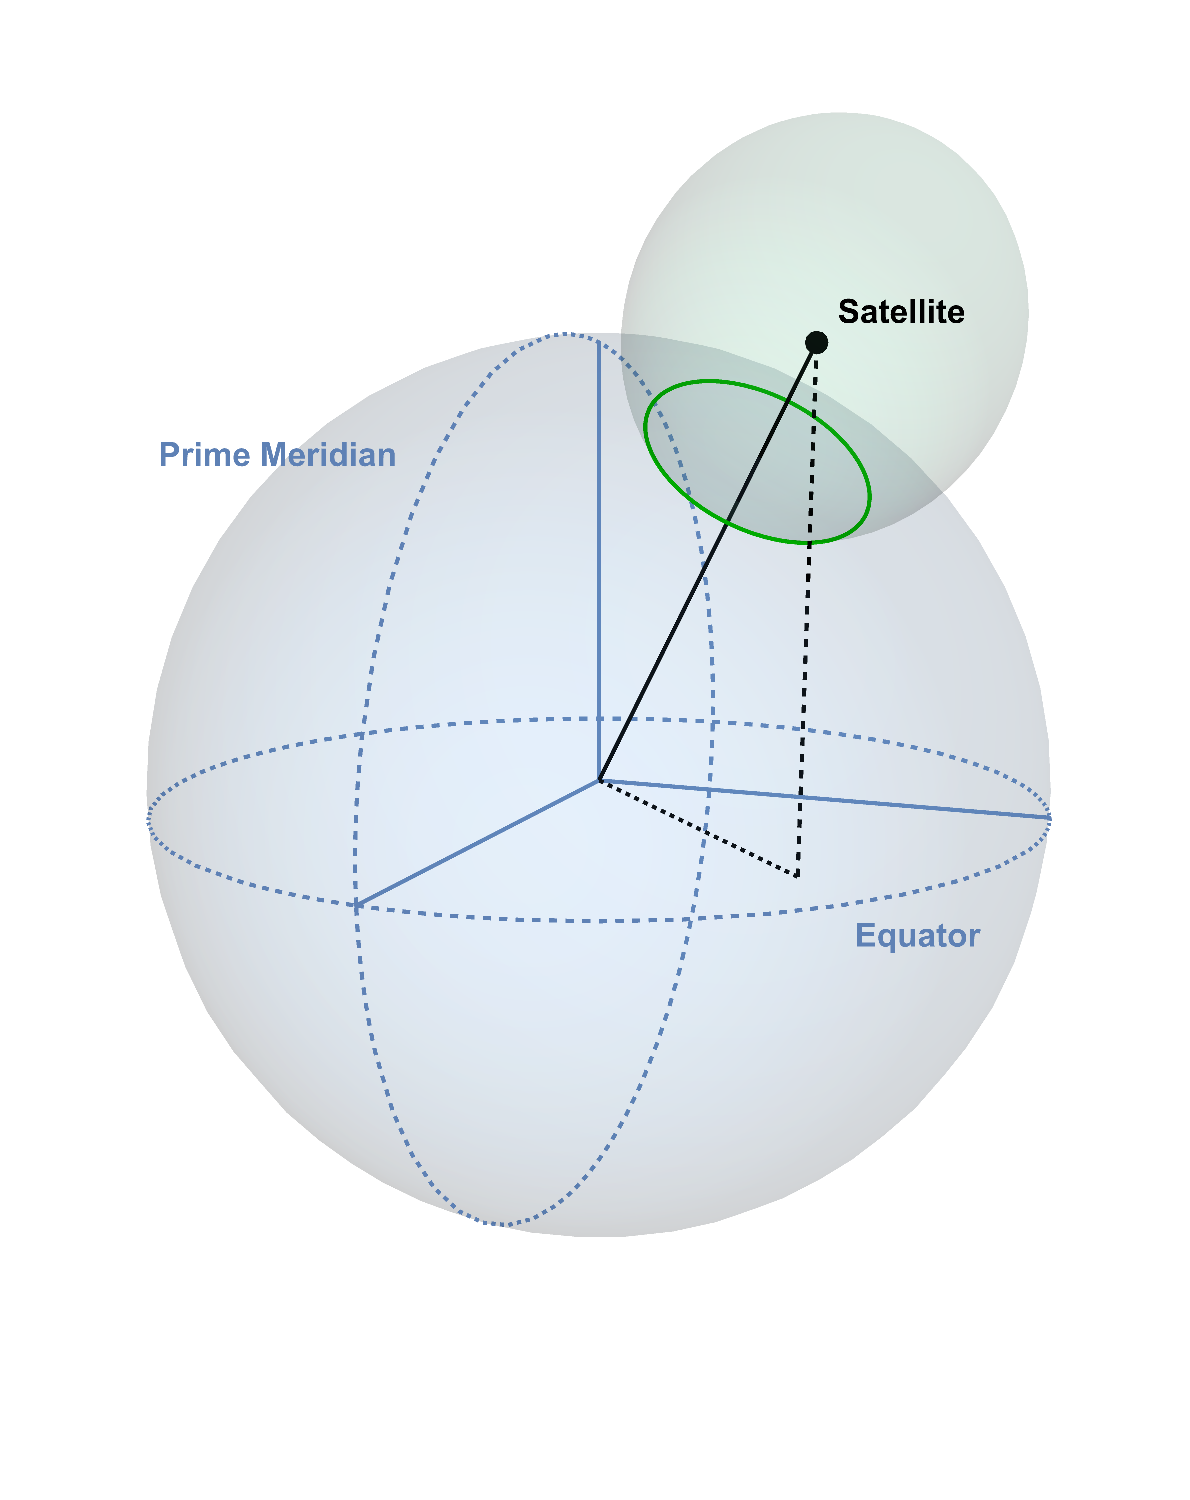
\includegraphics[clip, trim={2.4cm 4.4cm 1.6cm 3.5cm}, width=\textwidth * 35 / 100]{4 signal intersection.pdf}}%

  \onslide<4->{\vspace{0.25cm} Transit time $T$}
  \onslide<5->{$\Rightarrow$ distance $c T$}
\end{frame}

\begin{frame}
  \frametitle{The pseudorange equation}

  \begin{center}
    \only<1>{\[\sqrt{(X - x)^2 + (Y - y)^2 + (Z - z)^2} = c T\]}%
    \only<2>{\[\sqrt{(X - x)^2 + (Y - y)^2 + (Z - z)^2} - c T = 0\]}%
    \only<3>{\[\sqrt{(X - x)^2 + (Y - y)^2 + (Z - z)^2} - c (T - t) = 0\]}%
    \only<4>{\[\sqrt{(X - \textcolor{red}{x})^2 + (Y - \textcolor{red}{y})^2 + (Z - \textcolor{red}{z})^2} - c (T - \textcolor{red}{t}) = 0\]}%
    \only<5>{\[\sqrt{(\textcolor{red}{X} - x)^2 + (\textcolor{red}{Y} - y)^2 + (\textcolor{red}{Z} - z)^2} - c (\textcolor{red}{T} - t) = 0\]}%
  \end{center}

  \only<1-2>{where $(x, y, z)$ is our unknown location.}%
  \only<3->{where $(x, y, z)$ is our unknown location and $t$ is our clock bias.}
\end{frame}

\section{Satellite location and transit time}

\begin{frame}
  \frametitle{Transmission time}

  \centering
  \only<2,5>{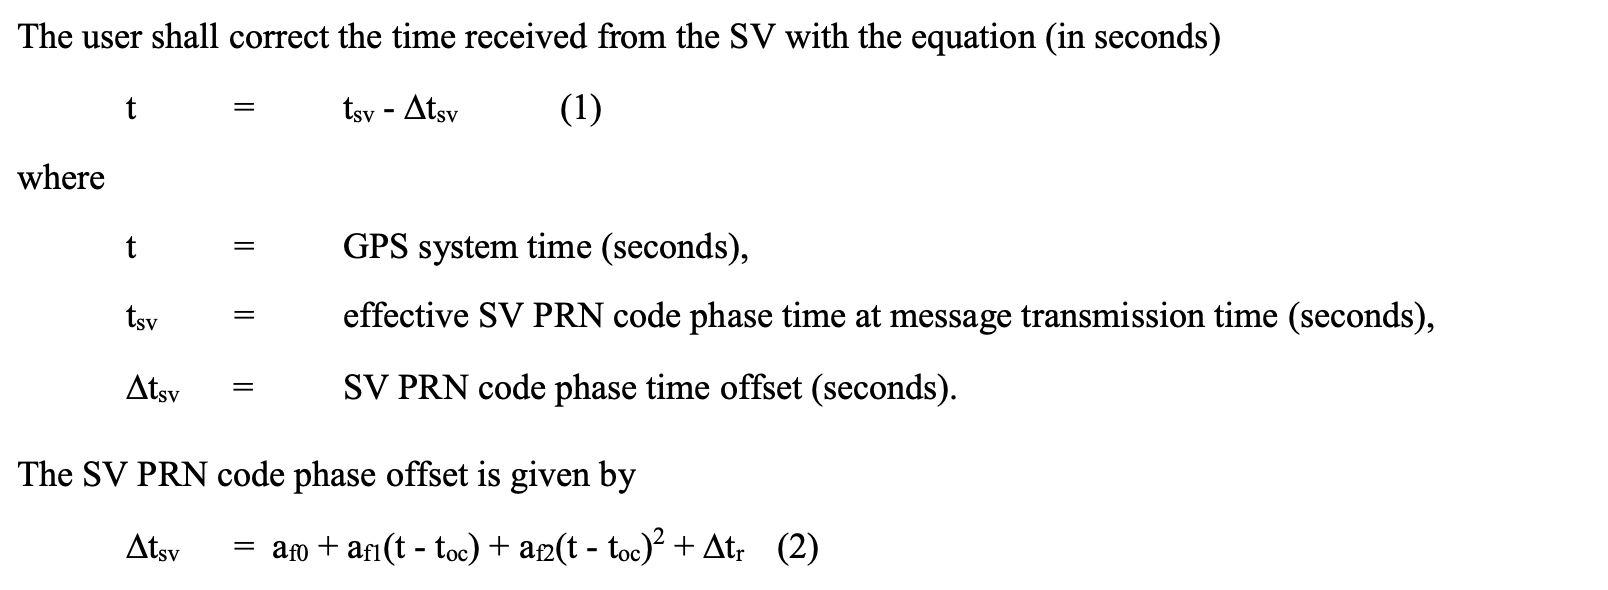
\includegraphics[width=\textwidth * 3 / 4]{5 transmission time.png}}%
  \only<3,6>{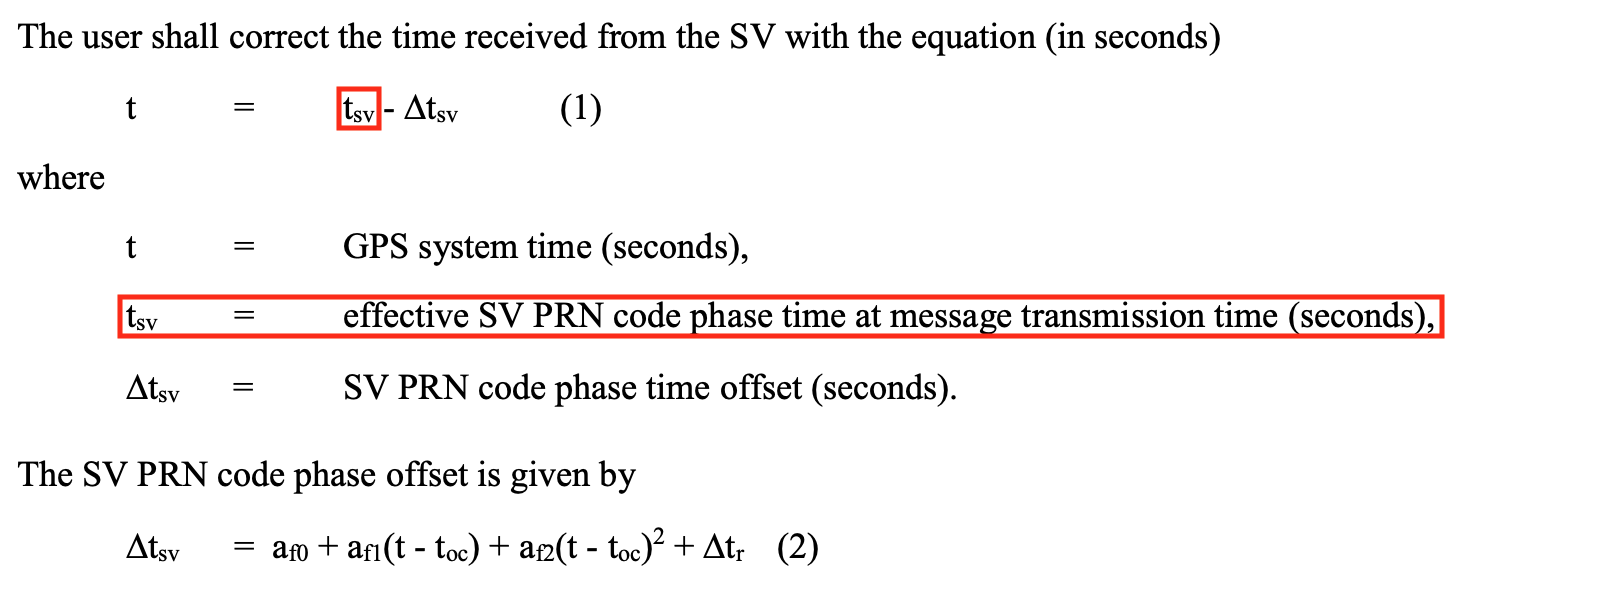
\includegraphics[width=\textwidth * 3 / 4]{7 tsv.png}}%
  \only<4>{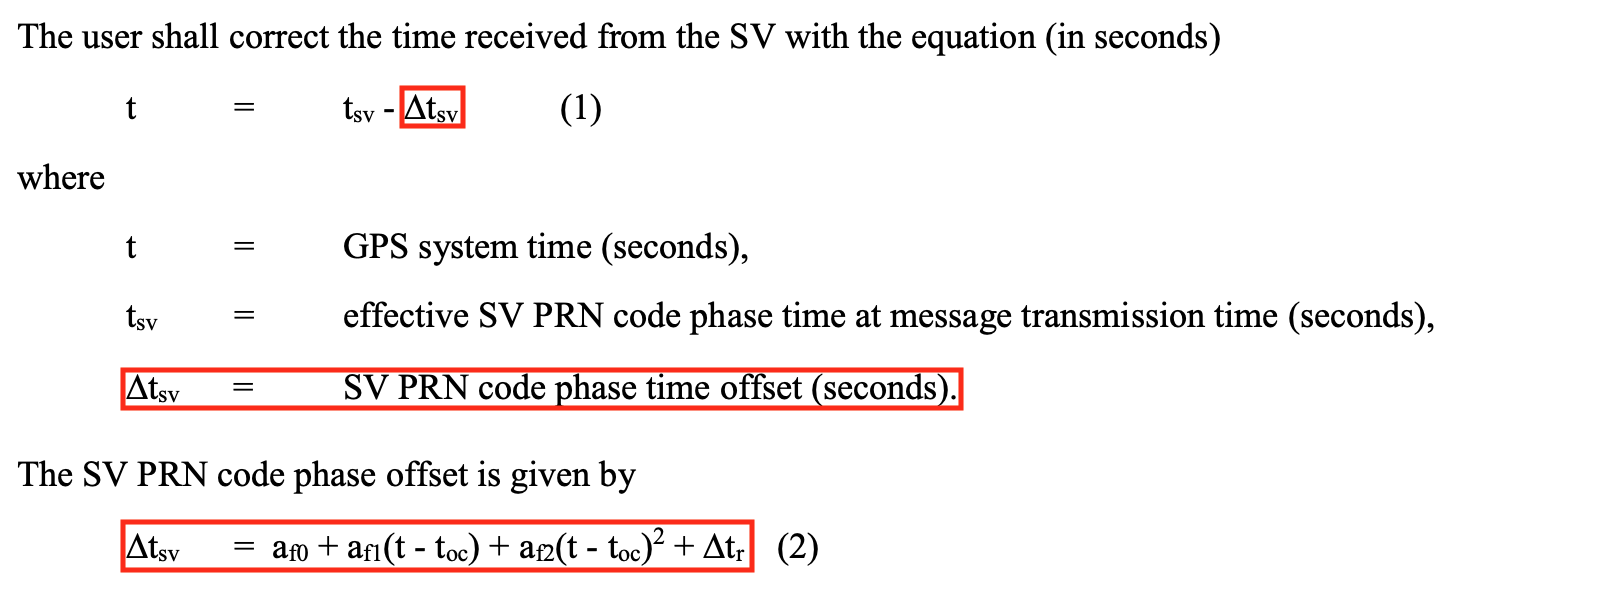
\includegraphics[width=\textwidth * 3 / 4]{8 delta tsv.png}}%
  \only<2->{\\ $\vdots$ \vspace{0.25cm} \\}
  \only<2-4,6>{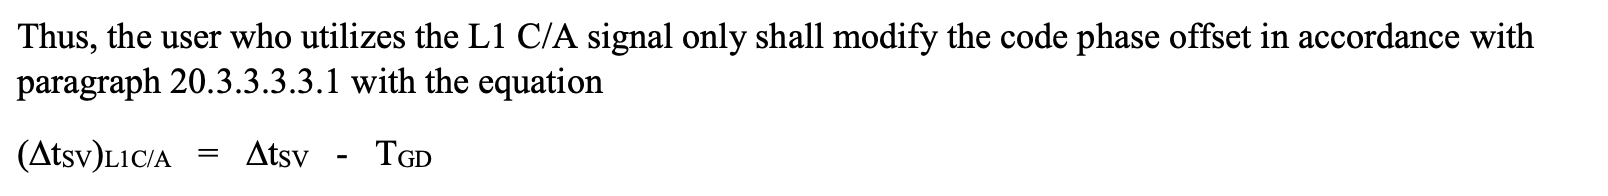
\includegraphics[width=\textwidth * 3 / 4]{6 l1 correction.png}}%
  \only<5>{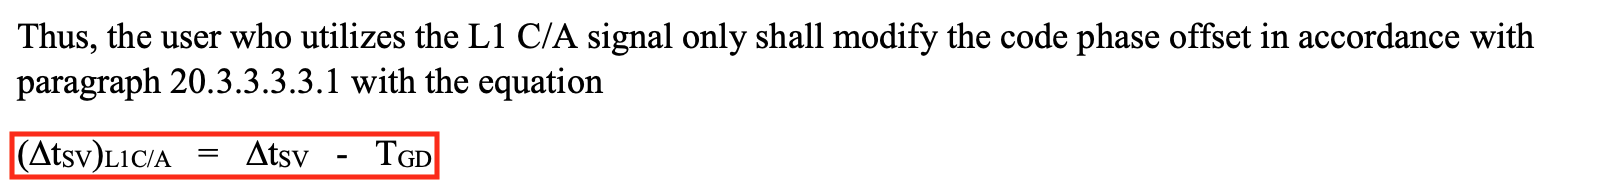
\includegraphics[width=\textwidth * 3 / 4]{9 l1 correction.png}}%
\end{frame}

\begin{frame}
  \frametitle{Transmission time}

  \centering
  \Large
  \[t_{sv} = \text{TOW} \times \qty{6}{s} \onslide<2->{+ \text{PRN count} \times \qty{1}{ms}}\]
\end{frame}

\begin{frame}
  \frametitle{Reception time}

  \begin{enumerate}
    \item<2-> Record the time at which we finish receiving the PRN code (our clock)
    
    \item<3-> Add 18 leap seconds
    
    \item<4-> Calculate the number of seconds since GPS started operating
    
    \item<5-> Calculate the remainder when divided by the number of seconds in a GPS week
  \end{enumerate}
\end{frame}

\begin{frame}
  \frametitle{Location}

  \centering
  \only<1>{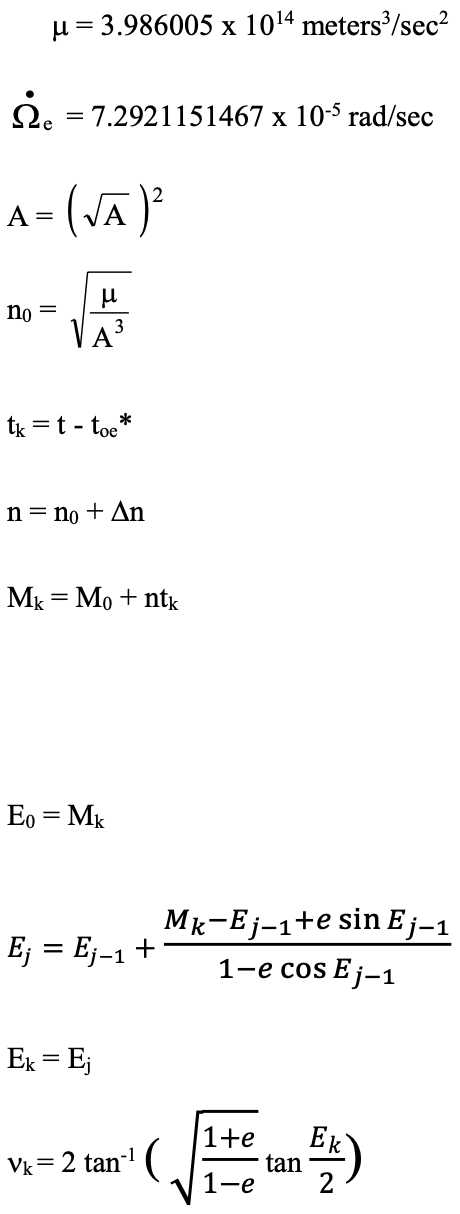
\includegraphics[width=\textwidth/6]{10 equations.png}}%
  \only<2>{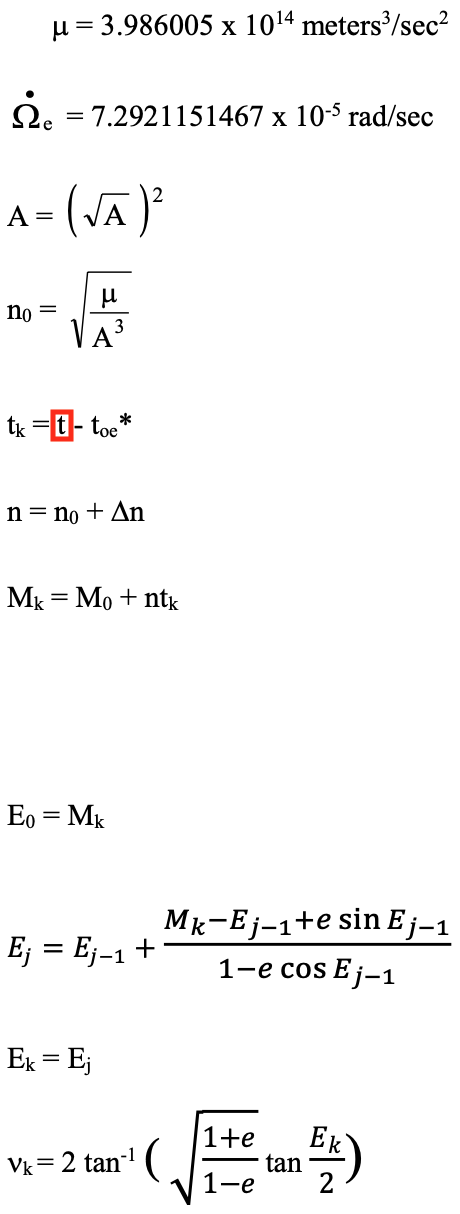
\includegraphics[width=\textwidth/6]{12 equations t.png}}%
  \hspace{0.5cm}%
  \raisebox{0.55\height}{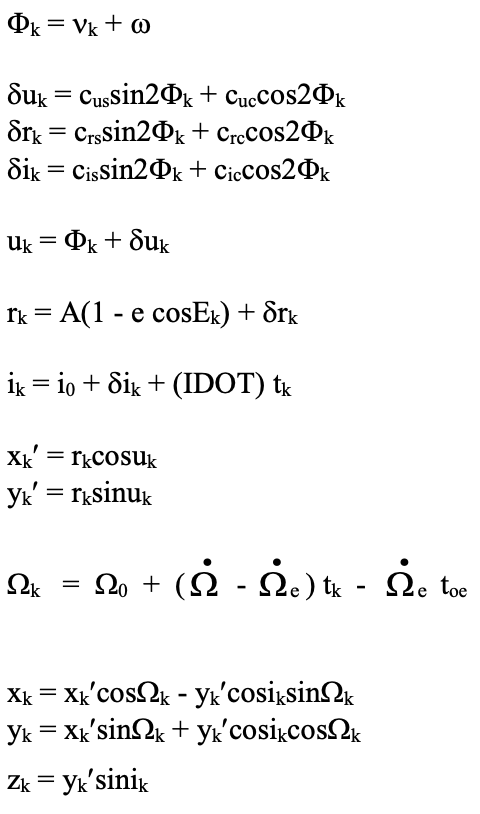
\includegraphics[width=\textwidth/6]{11 equations 2.png}}
\end{frame}

\begin{frame}
  \frametitle{The pseudorange equation}

  \[\sqrt{(X - x)^2 + (Y - y)^2 + (Z - z)^2} - c (T - t) = 0\]
\end{frame}

\section{System of equations}

\subsection{Definition}

\begin{frame}
  \frametitle{Definition}

  \begin{align*}
    \sqrt{(X_1 - x)^2 + (Y_1 - y)^2 + (Z_1 - z)^2} - c (T_1 - t) &= 0 \\
    \sqrt{(X_2 - x)^2 + (Y_2 - y)^2 + (Z_2 - z)^2} - c (T_2 - t) &= 0 \\
    \sqrt{(X_3 - x)^2 + (Y_3 - y)^2 + (Z_3 - z)^2} - c (T_3 - t) &= 0 \\
    \sqrt{(X_4 - x)^2 + (Y_4 - y)^2 + (Z_4 - z)^2} - c (T_4 - t) &= 0
  \end{align*}
\end{frame}

\subsection{Solving}

\begin{frame}
  \frametitle{The Newton-Raphson method}

  \centering
  \only<2>{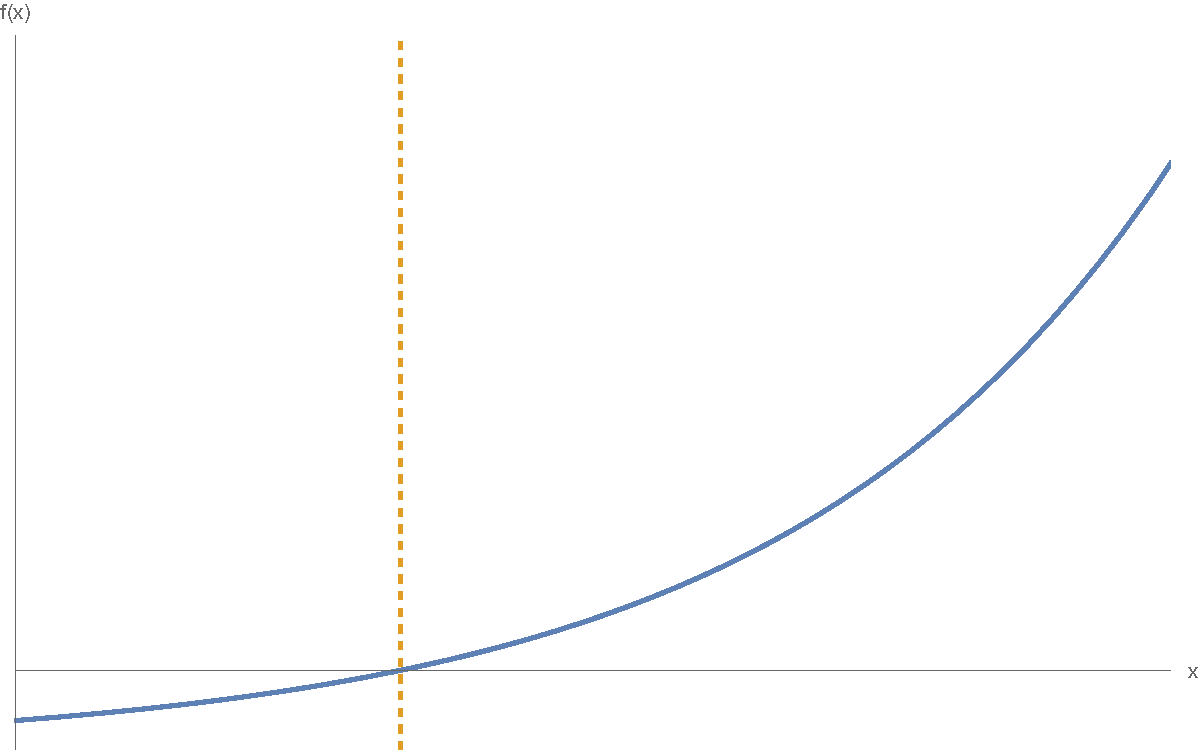
\includegraphics[width=\textwidth * 2 / 3]{13 newton raphson 1.pdf}}%
  \only<3>{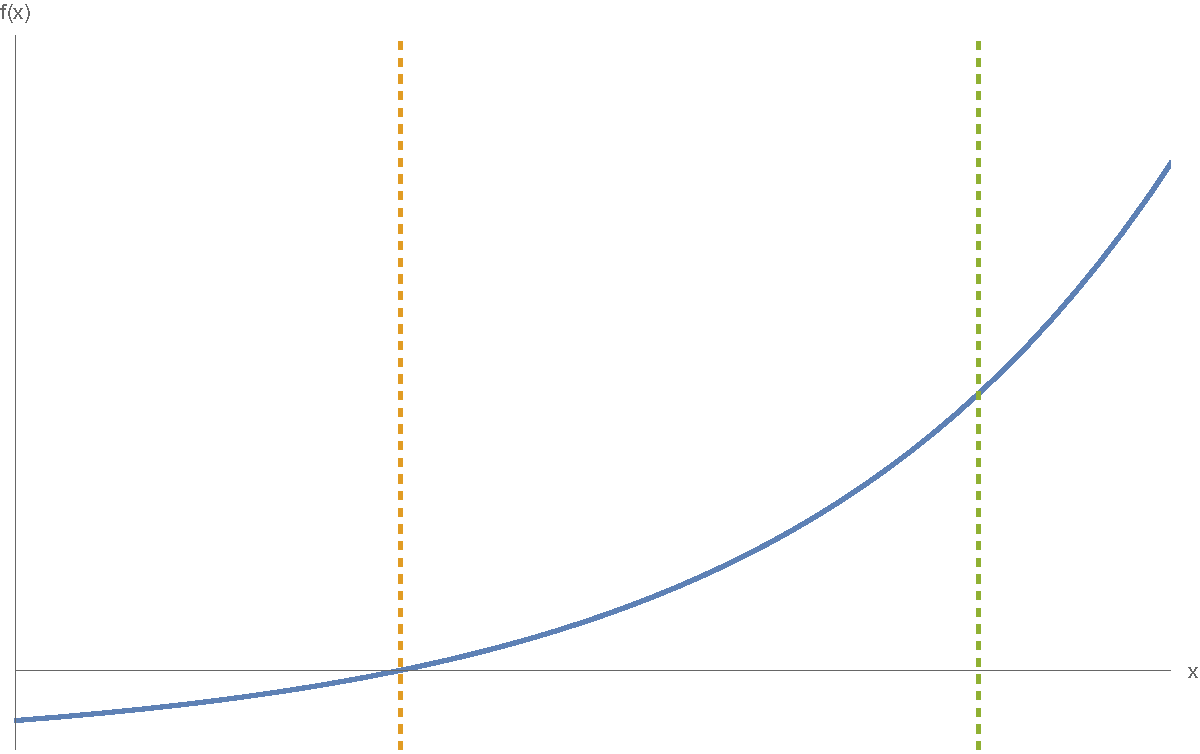
\includegraphics[width=\textwidth * 2 / 3]{14 newton raphson 2.pdf}}%
  \only<4>{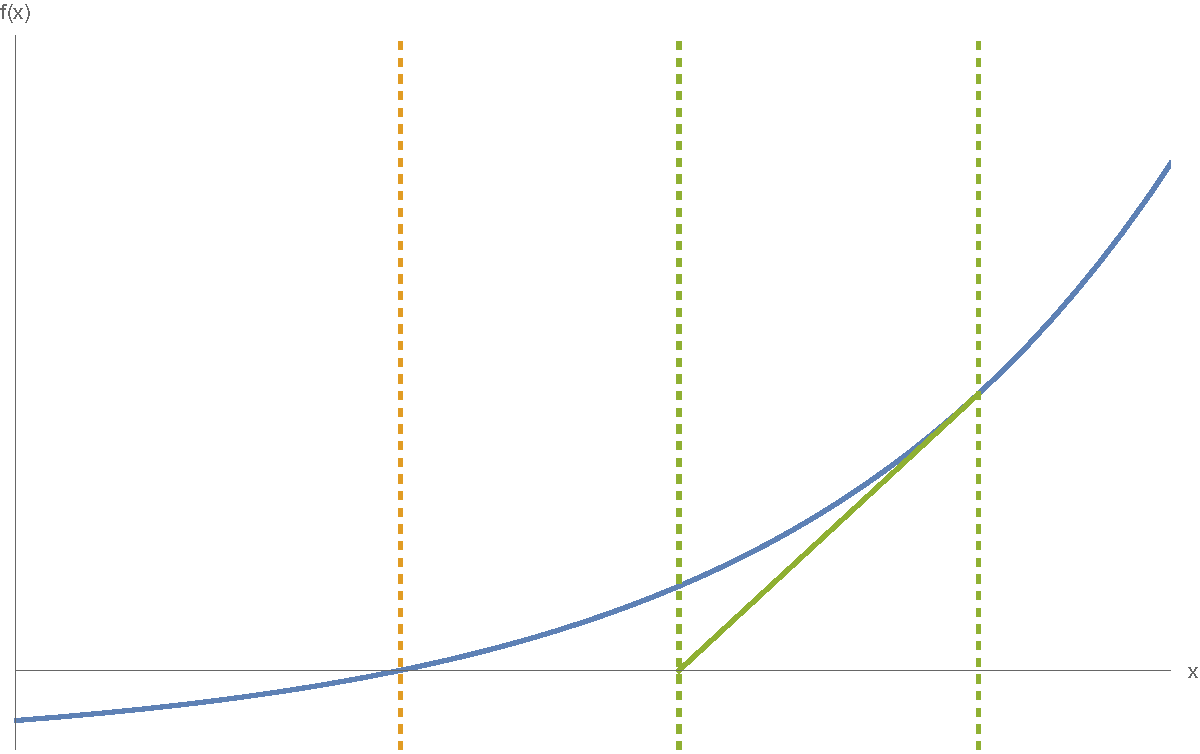
\includegraphics[width=\textwidth * 2 / 3]{15 newton raphson 3.pdf}}%
  \only<5>{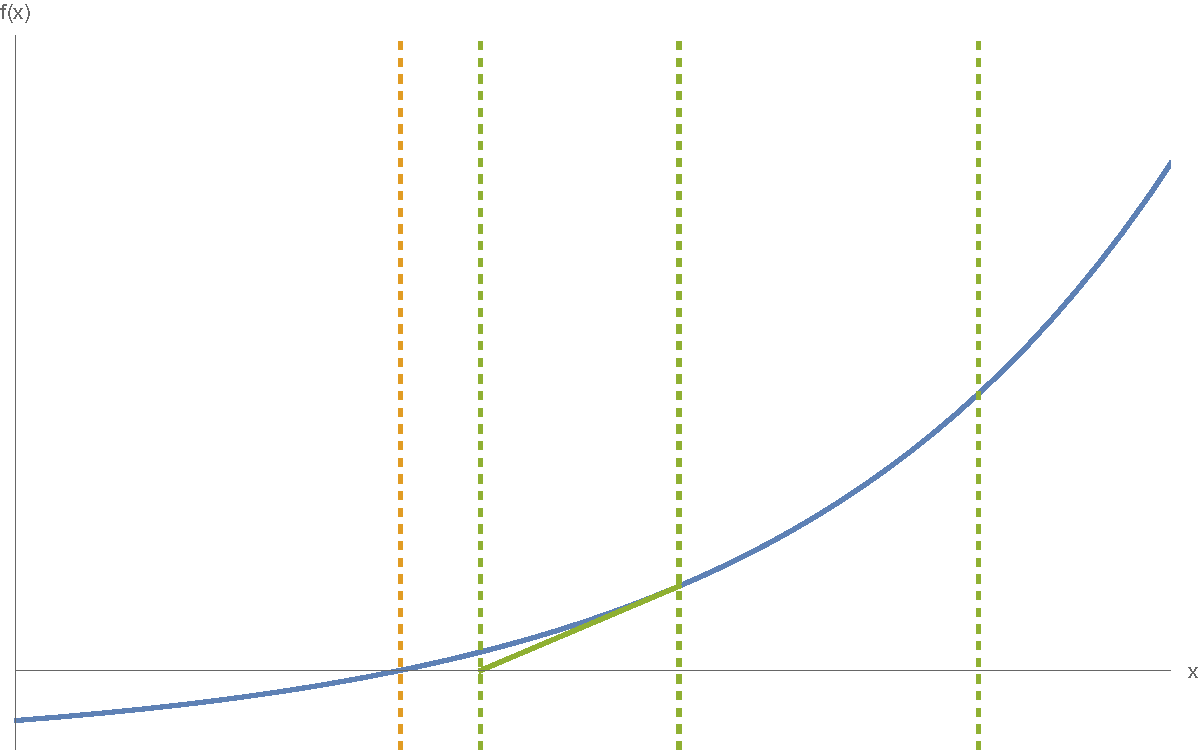
\includegraphics[width=\textwidth * 2 / 3]{16 newton raphson 4.pdf}}%
  \only<6>{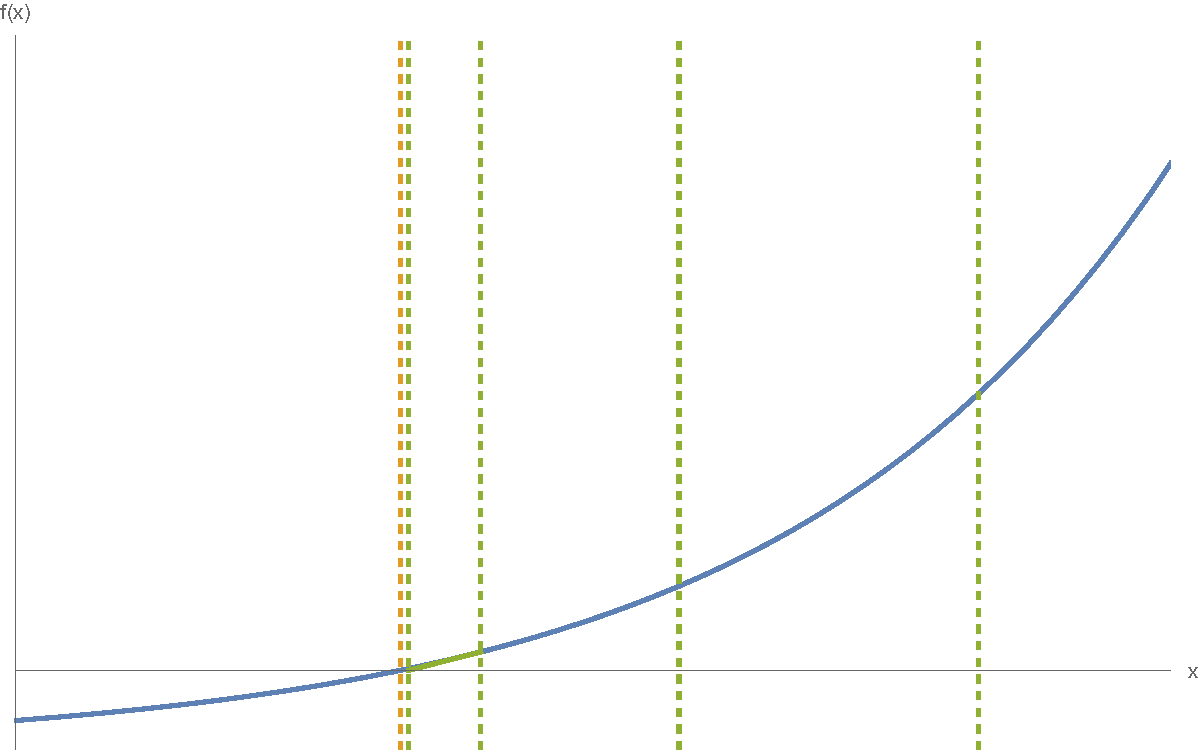
\includegraphics[width=\textwidth * 2 / 3]{17 newton raphson 5.pdf}}%
  \only<7>{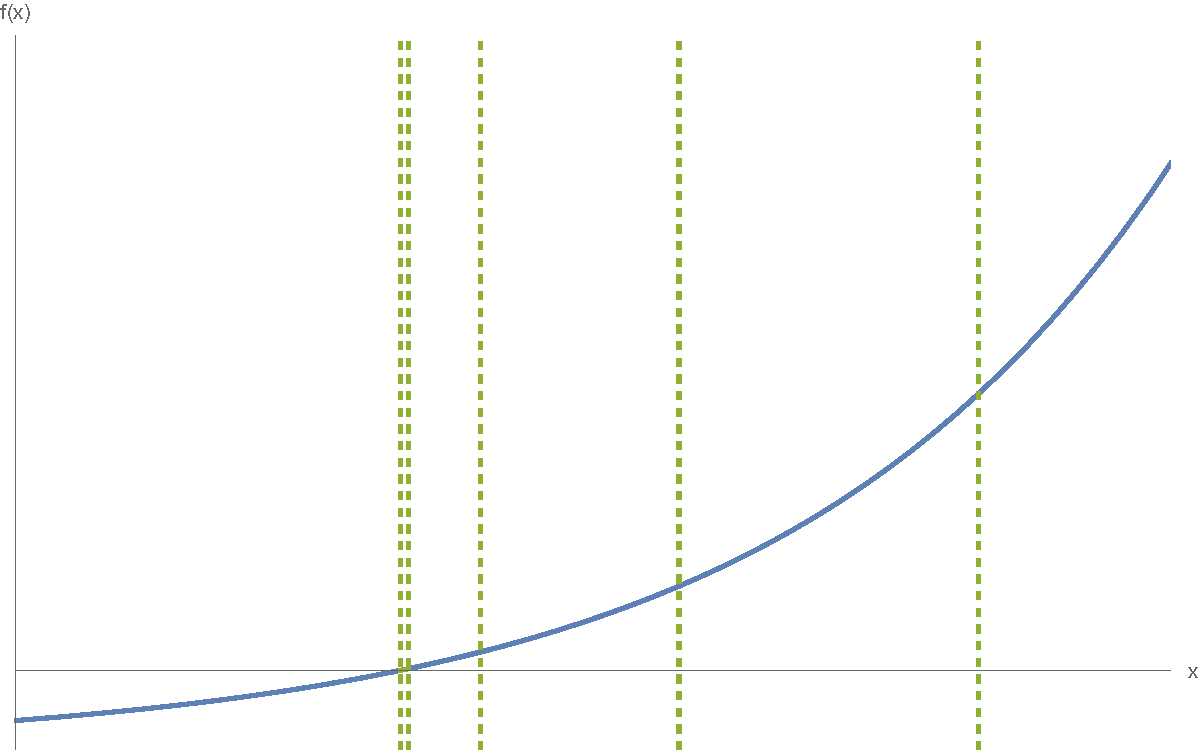
\includegraphics[width=\textwidth * 2 / 3]{18 newton raphson 6.pdf}}%
\end{frame}

\begin{frame}
  \frametitle{The Gauss-Newton algorithm}

  \begin{itemize}
    \item<2-> Tries to make our four (or more) pseudorange equations of four variables all equal zero
    
    \item<3-> Initial guess $\beta_0 = (x_0, y_0, z_0, t_0)$

    \item<4-> The Jacobian matrix $J$ is the multi-dimensional equivalent of the derivative
    
    \item<5-> Cell $i, j$ tells us how the result of equation $i$ would change if we changed variable $j$
    
    \item<6-> We iteratively improve the guess $\beta_{n + 1} = \beta_n - (J^T J)^{-1} J^T r(\beta_n)$ where $r(\beta)$ is the residual vector (a column vector containing the results of evaluating the pseudorange equations)
    
    \item<7-> Convert from ECEF to geodetic coordinates using Bowring's method
  \end{itemize}
\end{frame}

\begin{frame}
  \frametitle{Hooray!}

  \centering
  
\includegraphics[width=\textwidth * 2 / 5]{19 party.png}
\end{frame}

\begin{frame}
  \frametitle{Recap}

  \begin{itemize}
    \item<2-> We express locations using ECEF coordinates

    \item<3-> The pseudorange equation relates our distance to the satellite and the signal transit time \[\sqrt{(X - x)^2 + (Y - y)^2 + (Z - z)^2} - c (T - t) = 0\]
    
    \item<4-> The signal transit time is defined as $T = t_\text{received} - t_\text{transmitted}$
    
    \item<5-> The satellite's location can be calculated using equations in the GPS spec
    
    \item<6-> We need a system of at least four pseudorange equations to solve for $x, y, z,$ and $t$
    
    \item<7-> The Gauss-Newton algorithm is used to estimate $x, y, z,$ and $t$
  \end{itemize}
\end{frame}

\begin{frame}
  \frametitle{}

  \centering
  \vspace{1cm}
  {\Huge Thank you!} \\
  \vspace{1cm}
  \texttt{https://github.com/chrisdoble/gps-receiver}
\end{frame}

\end{document}